%
% body.tex
%
% Copyright © 2020 Libao Jin <jinlibao@outlook.com>
% Distributed under terms of the MIT license.
%
Please note that the deadline will be enforced as per the previous homework. Remember that you are allowed to work in teams of two on this assignment. You are encouraged to prepare your work in \LaTeX{}; a template will be provided to help you put it all together. If you choose  to submit a hard copy, you may submit only one copy for a team, indicating the names of both contributors. Online submission is encouraged, however, in that case both members of a team should submit the PDF file containing  their work and showing both their names.

\emph{All plots generated in this homework should have a title, legend, and labeled $x$ and $y$-axes.} \\[15pt]

\textbf{Instruction}

\begin{enumerate}[label={\arabic*.}]
  \item Go to \url{https://www.overleaf.com} and sign in (required).
  \item Open \href{https://www.overleaf.com/read/rqdhjmcwvxgz}{template}, click \emph{Menu} (up left corner), then \emph{Copy Project}.
  \item Go to \verb|LaTeX/meta.tex| (the file \verb|meta.tex| under the folder \verb|LaTeX|) to change the section and your name, e.g.,
    \begin{itemize}
      \item change title to \verb|\title{MATH 3340-01 Scientific Computing Homework 4}|
      \item change author to \verb|\author{Albert Einstein \& Carl F. Gauss}|
    \end{itemize}
  \item For Problem 1, you can either type the solution in \LaTeX{} or write it on the printout.
  \item For Problem 2, 3, 4, you need to write function/script files, store results to output files, and save graphs to figure files. Here are suggested names for function files, script files, output files, and figure files:
    \begin{table}[!hbtp]
      \centering
      % \caption{caption}
      % \label{tab:label}
      \begin{tabular}{cllll}
        \toprule
        Problem & Function File            & Script File     & Output File       & Figure File \\
        \midrule
        2       & \verb|newtonNonlinear.m| & \verb|hw4_p2.m| & \verb|hw4_p2.txt| &                   \\
        3       &                          & \verb|hw4_p3.m| & \verb|hw4_p3.txt| & \verb|hw4_p3.pdf| \\
        4       &                          & \verb|hw4_p4.m| & \verb|hw4_p4.txt| & \verb|hw4_p4.pdf| \\
        \bottomrule
      \end{tabular}
    \end{table}

    Once finished, you need to upload these files to the folder \verb|src| on Overleaf. If you have different filenames, please update the filenames in \verb|\lstinputlisting{../src/your_script_name.m}| accordingly. You can code in the provided files in \href{https://libaoj.in/courses/2021s/MATH3340/Homework/4/hw4.zip}{hw4.zip}, and use the MATLAB script \verb|save_results.m| to generate the output files and store the graphs to \verb|.pdf| files automatically (the script filenames should be exactly same as listed above).
  \item Recompile, download, and print out the generated PDF.
  \item You may find \href{https://libaoj.in/files/LaTeX.Mathematical.Symbols.pdf}{\LaTeX{}.Mathematical.Symbols.pdf} and the second part of \href{https://libaoj.in/courses/2021s/MATH3341/slides/Math.3341.Lab.01.Slides.pdf}{Lab 01 Slides} and \href{https://libaoj.in/courses/2021s/MATH3341/slides/Math.3341.Lab.02.Slides.pdf}{Lab 02 Slides} helpful.
\end{enumerate}
\newpage

%%%%%%%%%%%%%%%%%%%%%%%%%%%%%%%%%%%%%%%%%%%%%%%%
% Problem 1
%%%%%%%%%%%%%%%%%%%%%%%%%%%%%%%%%%%%%%%%%%%%%%%%
\section{Problem 1}%
\label{sec:problem_1}
Do by hand, on paper, one iteration of Newton's method for the nonlinear system:
\begin{equation*}
  \begin{cases}
    x^{2} + y^{3} - 1 = 0, \\
    x^{3} - y^{2} + 0.25 = 0.
  \end{cases}
\end{equation*}
Start with the initial guess $\mathbf{x}^{0} = [x^{0}, y^{0}]^{T} = [0.5, 0.5]^{T}$ and compute the next iterate $\mathbf{x}^{1}$. Also compare the norm of the residual at the new iterate with the residual norm computed for the initial guess.
\begin{solution}
  \quad \vfill % delete this line if you type the answer in LaTeX
\end{solution}

%%%%%%%%%%%%%%%%%%%%%%%%%%%%%%%%%%%%%%%%%%%%%%%%
% Problem 2
%%%%%%%%%%%%%%%%%%%%%%%%%%%%%%%%%%%%%%%%%%%%%%%%
\section{Problem 2}%
\label{sec:problem_2}
Solve the system
\begin{equation*}
  \begin{cases}
    10 - x + \sin(x + y) - 1 = 0 \\
    8 y - \cos^{2}(z - y) - 1 = 0 \\
    12 z + \sin(z) - 1 = 0
  \end{cases}
\end{equation*}
using a residual tolerance of $10^{-6}$ and the initial guess, $\mathbf{x}^{0} = [0.1, 0.25, 0.08]^{T}$. Print out the values for $x$, $y$, and $z$ for each iteration in a table similar to  the one you created for the problem of the previous  homework. You should submit your code (which can again be organized as a function and the script calling this function) together with your output.
\begin{solution}
  \quad
  \begin{itemize}
    \item
      Function file \verb|newtonNonlinear.m|
      \lstinputlisting[style=MATLAB]{../src/newtonNonlinear.m}
    \item
      Script file \verb|hw4_p2.m|
      \lstinputlisting[style=MATLAB]{../src/hw4_p2.m}
    \item
      Output file \verb|hw4_p2.txt|
      \lstinputlisting[style=Plain]{../src/hw4_p2.txt}
  \end{itemize}
\end{solution}

%%%%%%%%%%%%%%%%%%%%%%%%%%%%%%%%%%%%%%%%%%%%%%%%
% Problem 3
%%%%%%%%%%%%%%%%%%%%%%%%%%%%%%%%%%%%%%%%%%%%%%%%
\section{Problem 3}%
\label{sec:problem_3}
In a script file, find  an exponential fit of the form $f(x) = C e^{Ax}$ to the data (Table \ref{tab:p3}).
\begin{table}[!hbtp]
  \centering
  \caption{Problem 3 Data Points}
  \label{tab:p3}
  \begin{tabular}{ccccccc}
    \toprule
    $x$ & $0.0$   & $0.1$   & $0.2$   & $0.3$   & $0.4$   & $0.5$ \\
    \midrule
    $y$ & $1.388$ & $1.647$ & $1.951$ & $2.633$ & $3.321$ & $3.977$ \\
    \bottomrule
  \end{tabular}
\end{table}
Print your values for $A$ and $C$, then plot $f(x)$ vs. $x$ where \verb|x = 0:0.01:0.5| along with the original data points. Use a visible marker to mark the data points. Include the values of $A$ and $C$ in your report file along with the generated  plot and script file contained your code.
\begin{solution}
  \quad
  \begin{itemize}
    \item
      Script file \verb|hw4_p3.m|
      \lstinputlisting[style=MATLAB]{../src/hw4_p3.m}
    \item
      Output file \verb|hw4_p3.txt|
      \lstinputlisting[style=Plain]{../src/hw4_p3.txt}
      \begin{figure}[!hbtp]
        \centering
        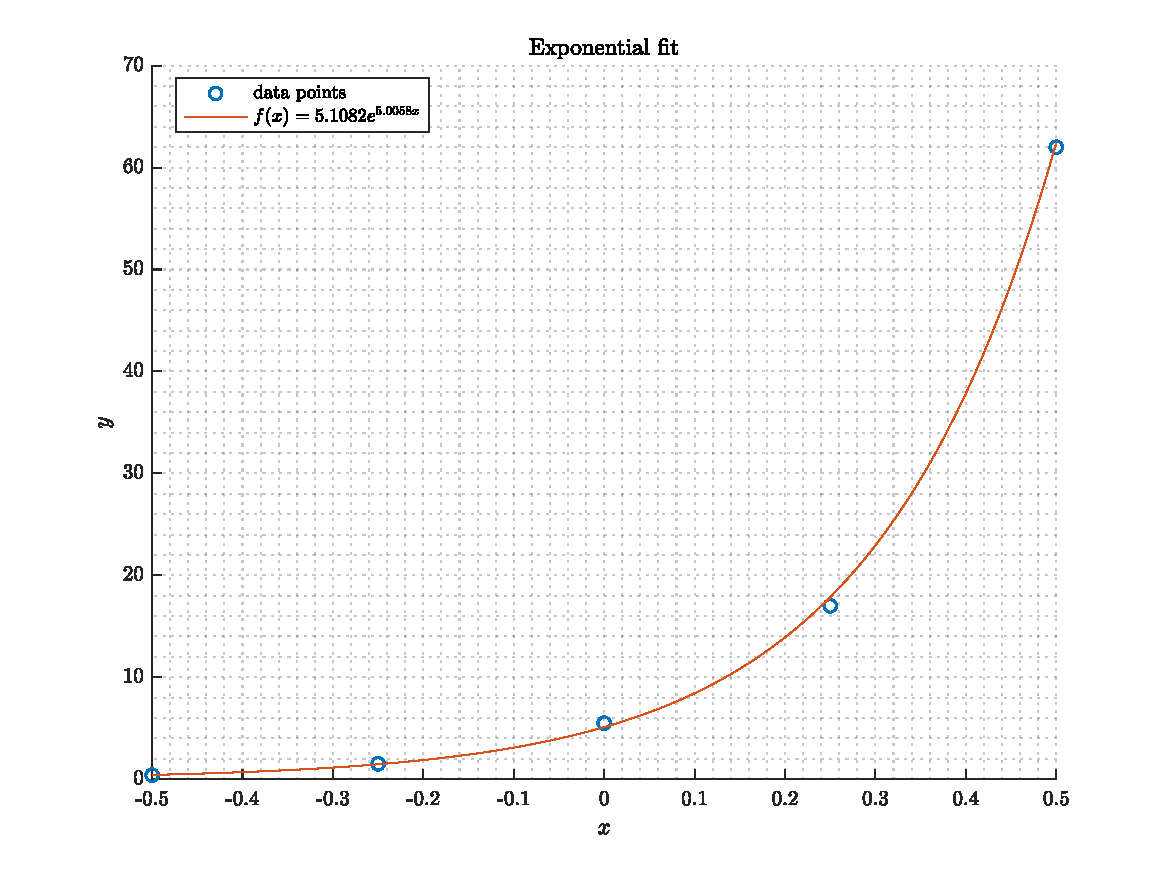
\includegraphics[width=0.8\linewidth]{../src/hw4_p3.pdf}
        \caption{}%
        \label{fig:}
      \end{figure}
  \end{itemize}
\end{solution}

%%%%%%%%%%%%%%%%%%%%%%%%%%%%%%%%%%%%%%%%%%%%%%%%
% Problem 4
%%%%%%%%%%%%%%%%%%%%%%%%%%%%%%%%%%%%%%%%%%%%%%%%
\section{Problem 4}%
\label{sec:problem_4}
Write a script file to find a quadratic fit of the form $f(x) = A x^{2} + B x + C$ to the data (Table \ref{tab:p4}).
\begin{table}[!hbtp]
  \centering
  \caption{Problem 4 Data Points}
  \label{tab:p4}
  \begin{tabular}{cccccc}
    \toprule
    $x$ & $0$     & $1$      & $2$      & $3$     & $4$ \\
    \midrule
    $y$ & $0.695$ & $-1.475$ & $-1.275$ & $0.882$ & $4.765$ \\
    \bottomrule
  \end{tabular}
\end{table}
Print your values for $A$, $B$, and $C$, then plot $f(x)$ vs $x$ where \verb|x = 0:0.1:4| along with the original data  points. Use a visible marker for the data points. Include the values of $A$, $B$, and $C$ in your report file along with the generated plot and script file containing your code.
\begin{solution}
  \quad
  \begin{itemize}
    \item
      Script file \verb|hw4_p4.m|
      \lstinputlisting[style=MATLAB]{../src/hw4_p4.m}
    \item
      Output file \verb|hw4_p4.txt|
      \lstinputlisting[style=Plain]{../src/hw4_p4.txt}
      \begin{figure}[!hbtp]
        \centering
        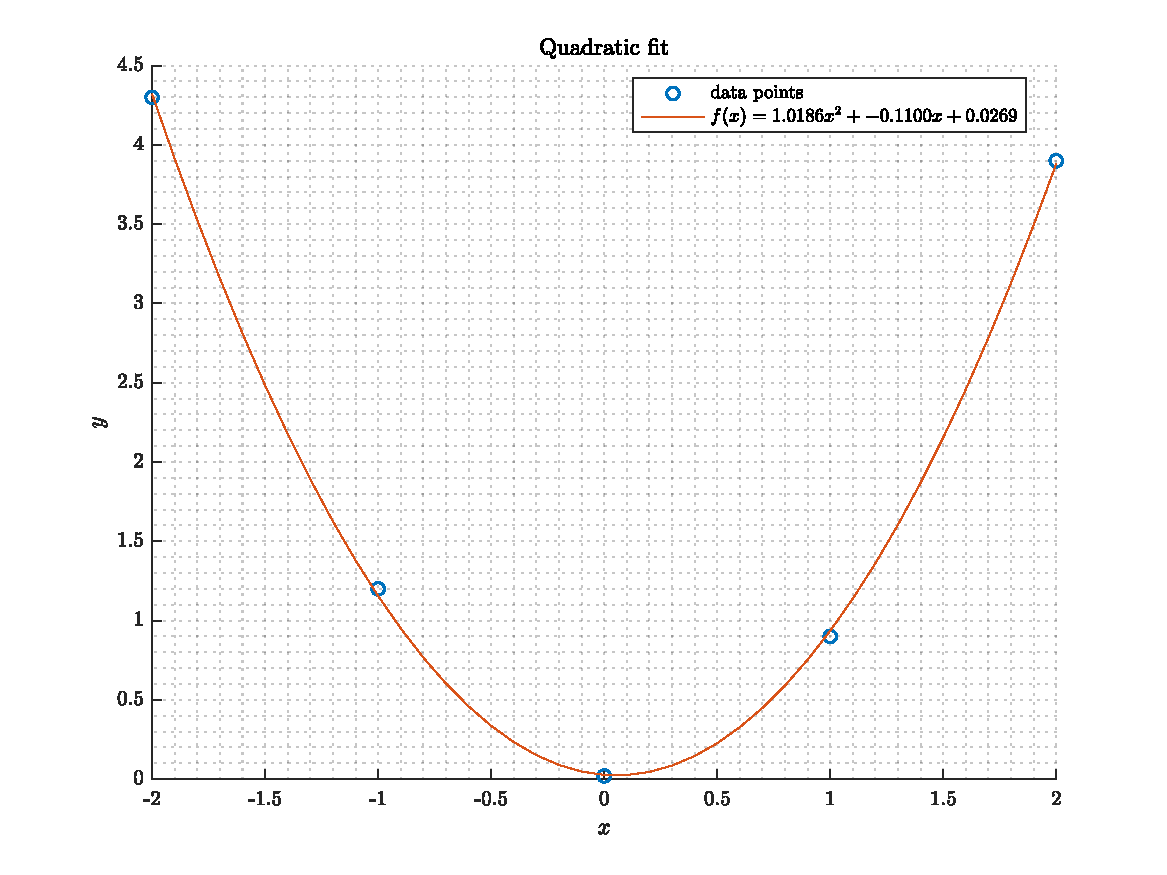
\includegraphics[width=0.8\linewidth]{../src/hw4_p4.pdf}
        \caption{}%
        \label{fig:}
      \end{figure}
  \end{itemize}
\end{solution}
